\documentclass[aspectratio=169,11pt]{beamer}
\usetheme{Boadilla}
\usecolortheme{default}
\setbeamertemplate{navigation symbols}{}
\setbeamertemplate{footline}[frame number]
\usepackage[utf8]{inputenc}
\usepackage{tikz}
\usepackage{booktabs}
\usepackage{array}

\title{How Did Expanding Universities Change\\ Who Gets a Good Job in Iran?}
\subtitle{Educational mismatch, the gender employment gap, and university access}
\author{Mahyar Rezazadeh \and Hossein Jalili}
\date{August 2026}

\begin{document}

% ---------- Slide 1: Title ----------
\begin{frame}
\titlepage
\end{frame}

% ---------- Slide 2: The Question ----------
\begin{frame}[c]{The Big Picture}
\begin{itemize}
\item Between the mid-1990s and mid-2010s, Iran expanded its universities faster than almost any country in the world --- from a small, exam-selected elite system to one that now credentials roughly \textbf{one in three} employed workers.
\medskip
\item Two questions this project answers:
\begin{enumerate}
\item Did more university access mean more people ended up \textbf{working}, and working in a job that actually \textbf{matches their training}?
\item Does the answer look the same for \textbf{women} as for \textbf{men}?
\end{enumerate}
\end{itemize}
\end{frame}

% ---------- Slide 3: The Data ----------
\begin{frame}[c]{The Data: Iran's Labor Force Survey}
\begin{itemize}
\item \textbf{Source:} Iran's quarterly household Labor Force Survey (LFS), Persian years 1386--1403 ($\approx$ 2007--2025), 18 survey waves.
\medskip
\item \textbf{Size:} 4.13 million individual survey responses.
\medskip
\item \textbf{Geography:} 28 ``historical'' provinces --- boundaries adjusted so that administrative redrawing over time doesn't get mistaken for a real effect.
\medskip
\item \textbf{Who's in the sample:} people born 1355--1383, so that we can observe how much university capacity existed in their home province exactly when they were 18--20 years old --- the typical age of starting university.
\end{itemize}
\end{frame}

% ---------- Slide 4: The Design ----------
\begin{frame}{The Idea: Comparing People Who Only Differ in Local University Access}
\begin{block}{In plain words}
We compare people from the \textbf{same province}, born in the \textbf{same year}, surveyed in the \textbf{same year}. The one thing that differs between them: how many university seats (per 100,000 people) existed in their home province when they turned 18--20 --- what we call their \textbf{``university exposure.''}
\end{block}
\medskip
This strips out generic province differences (richer vs.\ poorer regions) and generic time trends (the whole economy improving or worsening), isolating the effect of \emph{local university access itself}.
\medskip
\begin{block}{For the technically curious}
\footnotesize
$Y_{ipct} = \beta \cdot \log(\text{Exposure}_{pc}) + X_i'\gamma + \mu_p + \lambda_c + \tau_t + \varepsilon_{ipct}$ \\
Survey-weighted; province ($\mu_p$), birth-cohort ($\lambda_c$), and survey-year ($\tau_t$) fixed effects; standard errors two-way clustered by province and cohort (28 $\times$ 29 clusters).
\end{block}
\end{frame}

% ---------- Slide 5: The Measures ----------
\begin{frame}[c]{What We Measured}
\begin{columns}[T]
\column{0.5\textwidth}
\textbf{Employment}\\
{\small Simply: are you working, or looking for work?}
\vspace{0.6cm}

\textbf{Vertical mismatch (over-education)}\\
{\small Are you more educated than your job typically calls for? (Benchmark: the most common education level among people in that occupation.)}

\column{0.5\textwidth}
\textbf{Horizontal mismatch}\\
{\small Are you working in a field unrelated to what you studied?}
\vspace{0.6cm}

\textbf{Double mismatch / fully matched}\\
{\small Both problems at once --- or neither.}
\end{columns}
\end{frame}

% ---------- Slide 6: Result 1 ----------
\begin{frame}{Result 1: More Universities Didn't Create More Jobs --- It Created Worse Matches}
\small
\begin{itemize}
\item Employment and labor-force participation: \textbf{no significant change} on average.
\item But job \emph{matching} got worse. Bars below: effect of a 10\% increase in local university exposure, in percentage points (pp).
\end{itemize}
\vspace{-0.4cm}
\begin{center}
\scalebox{0.56}{
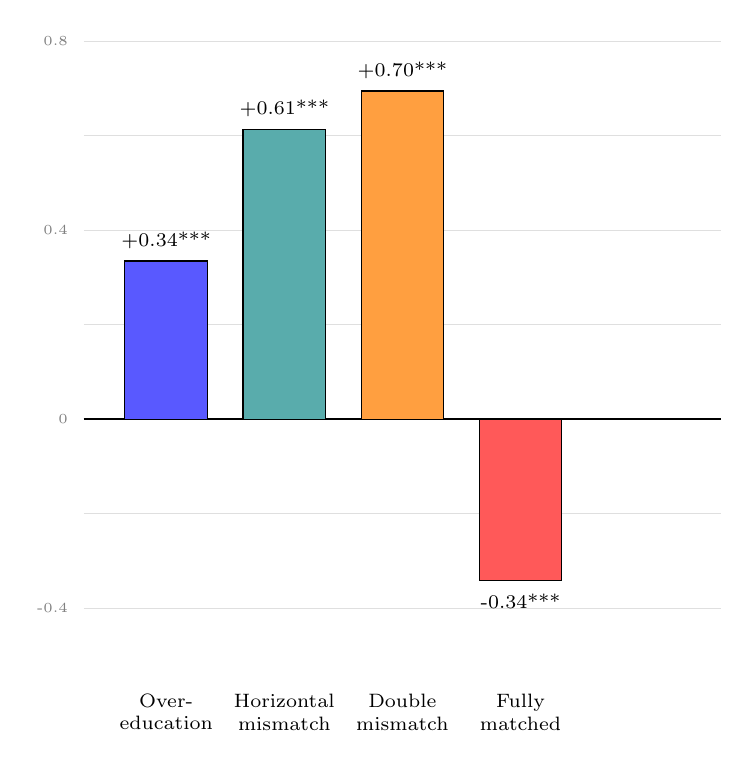
\begin{tikzpicture}[x=1.5cm,y=6cm]
\foreach \y in {-0.4,-0.2,0,0.2,0.4,0.6,0.8} {
  \draw[gray!25] (0.3,\y) -- (5.7,\y);
}
\node[left,font=\tiny,gray] at (0.25,0.8) {0.8};
\node[left,font=\tiny,gray] at (0.25,0.4) {0.4};
\node[left,font=\tiny,gray] at (0.25,0) {0};
\node[left,font=\tiny,gray] at (0.25,-0.4) {-0.4};
\draw[thick] (0.3,0) -- (5.7,0);
% Bar 1: Overeducation
\draw[fill=blue!65] (1-0.35,0) rectangle (1+0.35,0.335);
\node[above,font=\scriptsize] at (1,0.34) {+0.34***};
% Bar 2: Horizontal
\draw[fill=teal!65] (2-0.35,0) rectangle (2+0.35,0.614);
\node[above,font=\scriptsize] at (2,0.62) {+0.61***};
% Bar 3: Double
\draw[fill=orange!75] (3-0.35,0) rectangle (3+0.35,0.695);
\node[above,font=\scriptsize] at (3,0.70) {+0.70***};
% Bar 4: Fully matched
\draw[fill=red!65] (4-0.35,-0.341) rectangle (4+0.35,0);
\node[below,font=\scriptsize] at (4,-0.35) {-0.34***};
% category labels
\node[align=center,font=\scriptsize] at (1,-0.62) {Over-\\education};
\node[align=center,font=\scriptsize] at (2,-0.62) {Horizontal\\mismatch};
\node[align=center,font=\scriptsize] at (3,-0.62) {Double\\mismatch};
\node[align=center,font=\scriptsize] at (4,-0.62) {Fully\\matched};
\end{tikzpicture}
}
\end{center}
\vspace{-0.2cm}
{\scriptsize *** / ** / * denote statistical significance at the 1\% / 5\% / 10\% level. Pooled sample.}
\end{frame}

% ---------- Slide 7: Result 2 - gender puzzle ----------
\begin{frame}{Result 2: A Gender Puzzle}
\begin{center}
\scalebox{0.68}{
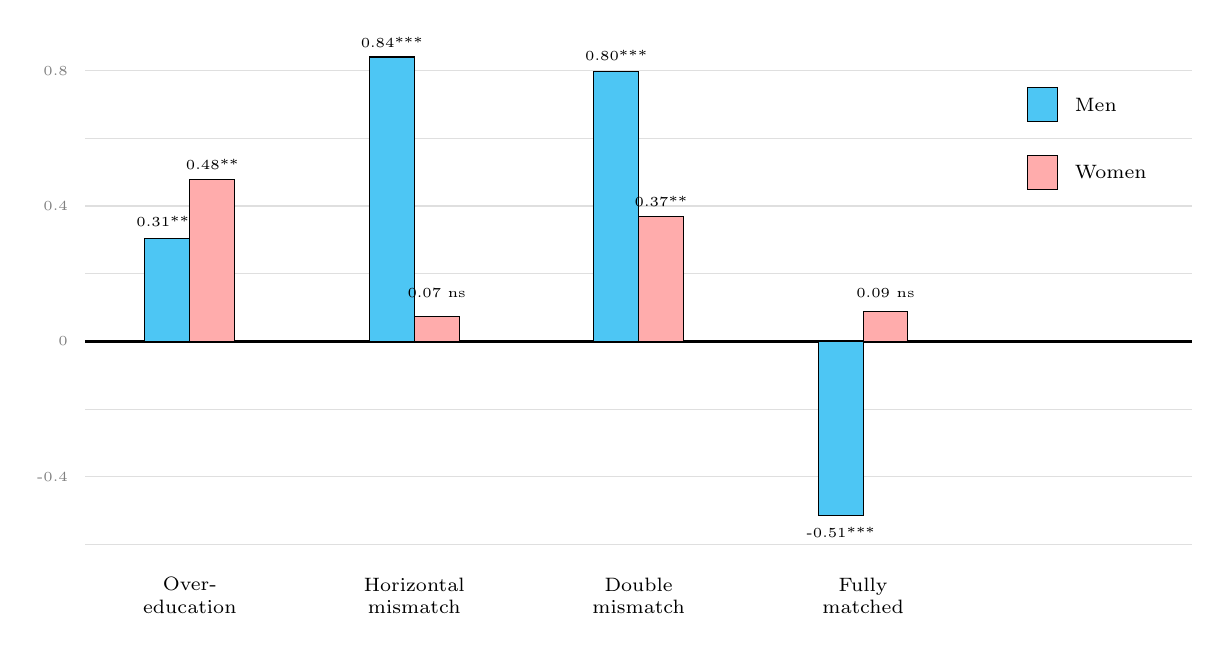
\begin{tikzpicture}[x=1.9cm,y=4.3cm]
\foreach \y in {-0.6,-0.4,-0.2,0,0.2,0.4,0.6,0.8} {
  \draw[gray!25] (0.3,\y) -- (7.7,\y);
}
\node[left,font=\tiny,gray] at (0.25,0.8) {0.8};
\node[left,font=\tiny,gray] at (0.25,0.4) {0.4};
\node[left,font=\tiny,gray] at (0.25,0) {0};
\node[left,font=\tiny,gray] at (0.25,-0.4) {-0.4};
\draw[thick] (0.3,0) -- (7.7,0);
% Group 1: Overeducation  Men 0.305 / Women 0.478
\draw[fill=cyan!70] (1-0.3,0) rectangle (1,0.305);
\node[above,font=\tiny] at (0.85,0.31) {0.31***};
\draw[fill=pink!90!red] (1,0) rectangle (1+0.3,0.478);
\node[above,font=\tiny] at (1.15,0.48) {0.48**};
% Group 2: Horizontal Men 0.840 / Women 0.073
\draw[fill=cyan!70] (2.5-0.3,0) rectangle (2.5,0.840);
\node[above,font=\tiny] at (2.35,0.84) {0.84***};
\draw[fill=pink!90!red] (2.5,0) rectangle (2.5+0.3,0.073);
\node[above,font=\tiny] at (2.65,0.10) {0.07 ns};
% Group 3: Double Men 0.797 / Women 0.368
\draw[fill=cyan!70] (4-0.3,0) rectangle (4,0.797);
\node[above,font=\tiny] at (3.85,0.80) {0.80***};
\draw[fill=pink!90!red] (4,0) rectangle (4+0.3,0.368);
\node[above,font=\tiny] at (4.15,0.37) {0.37**};
% Group 4: Fully matched Men -0.513 / Women 0.088
\draw[fill=cyan!70] (5.5-0.3,-0.513) rectangle (5.5,0);
\node[below,font=\tiny] at (5.35,-0.52) {-0.51***};
\draw[fill=pink!90!red] (5.5,0) rectangle (5.5+0.3,0.088);
\node[above,font=\tiny] at (5.65,0.10) {0.09 ns};
% category labels
\node[align=center,font=\scriptsize] at (1,-0.75) {Over-\\education};
\node[align=center,font=\scriptsize] at (2.5,-0.75) {Horizontal\\mismatch};
\node[align=center,font=\scriptsize] at (4,-0.75) {Double\\mismatch};
\node[align=center,font=\scriptsize] at (5.5,-0.75) {Fully\\matched};
% legend
\draw[fill=cyan!70] (6.6,0.75) rectangle (6.8,0.65);
\node[right,font=\scriptsize] at (6.85,0.70) {Men};
\draw[fill=pink!90!red] (6.6,0.55) rectangle (6.8,0.45);
\node[right,font=\scriptsize] at (6.85,0.50) {Women};
\end{tikzpicture}
}
\end{center}
\vspace{-0.3cm}
{\footnotesize Horizontal and double mismatch rise almost only for \textbf{men}. Over-education rises more for \textbf{women}. Why would expansion barely touch women's job matches, yet hit men hard?}
\end{frame}

% ---------- Slide 8: Solving the puzzle ----------
\begin{frame}{Solving the Puzzle: Who Actually Gets Counted as ``Employed''?}
\begin{itemize}
\item Only \textbf{15\%} of women in our sample work, versus \textbf{70\%} of men --- a 55-point gap.
\medskip
\item Among the women who \emph{do} work, they are noticeably more educated than the typical working-age woman, in every part of the exposure range.
\item Among men, working men look just like the average working-age man --- almost no such gap.
\medskip
\item One summary number (from a statistical selection-correction model): the link between ``getting to work at all'' and unobserved personal strengths is \textbf{5 times larger for women} than for men.
\end{itemize}
\begin{block}{The takeaway}
Women aren't protected from bad job matches by university expansion. We mostly just don't \emph{observe} most women working at all --- and the few who do work are an unusually strong, hand-picked group.
\end{block}
\end{frame}

% ---------- Slide 9: How big ----------
\begin{frame}[c]{How Much Does This Explain?}
\begin{itemize}
\item \textbf{Whether women work at all:} this selectivity difference explains only about \textbf{7.5\%} of why so few women work. The rest is something else --- social norms, institutions, or employer demand --- not women's own qualifications.
\medskip
\item \textbf{How much working women work:} among people who \emph{do} work, selection differences alone account for \emph{more} hours than the entire observed gender gap in weekly hours (33 hours of ``selection effect'' vs.\ a 14-hour raw gap).
\medskip
\item \textbf{Corroborating evidence:} the share of women among national university entrance exam takers rose from \textbf{59\%} (2014) to \textbf{63\%} (2024) --- women's access and ambition are rising, not falling.
\end{itemize}
\end{frame}

% ---------- Slide 10: Bottom line ----------
\begin{frame}{Bottom Line}
\begin{itemize}
\item Expanding universities pushed a real, growing share of \textbf{men} into jobs that don't match their training --- a genuine cost of fast-paced expansion.
\medskip
\item It didn't do the same to \textbf{women} on paper --- but only because Iran's labor market keeps the vast majority of women out of employment altogether, admitting only an unusually well-qualified few.
\medskip
\item This points to a \textbf{demand-constrained} story: the binding constraint sits on the labor-market side, not on women's education or effort.
\end{itemize}
\vspace{0.4cm}
\begin{block}{Two connected papers}
\small The core mismatch paper (\emph{University Expansion, Educational Mismatch, and Occupational Allocation in Iran}) and a follow-up on gender selection (\emph{University Access, Educational Mismatch, and the Selective Gender Gap in Iran's Labor Market}, prepared for the \emph{International Labour Review}).
\end{block}
\end{frame}

\end{document}
